\chapter{Methods}
\section{Distance Function}
\subsection{Motivation}
In chapter \ref{loss_landscape}, we got a brief overview over the loss landscape
of deep neural networks and the resulting challenges for optimization. Although
there exists a large number of local minima, most of them have low cost.
Furthermore, they are arranged in cells, where each minima has low cost and is
connected to the others via valleys of low loss.

These cells create a challenge for optimization. Suppose the learning gets into
the area of one of these cells. As mentioned in chapter \ref{loss_landscape} the
cells are surrounded by nondifferential boundaries and areas of higher loss.
[TODO: where is this stated?] This will likely cause the algorithm to get stuck
into this cells. As all of the minimas in this cell are of approximatly same
loss, there will be a boundary until the algorithm can improve, which may be
higher than the global optimum. This also poses the question, if continuing to
train is useful, as after one of the minima in the cell is found, the nearby
minima ic can reach will offer no significant improvement.

How to overcome this issue? One solution would be to escape these cells and move
to the next one, hopefully with lower cost. This can be achieved with the use of
warm restarts, as mentioned in chapter \ref{cosine_decay}. In phases of low
learning rate, the algorithm exploits the area of a cell. When the learning rate
is set back up to the inital learning rate, the update steps of the parameters
get much larger. If the update steps are large enough, this may lead to an
escape of the cell. However there is no guarantee, because this method relies on
the gradient beeing large enough.

From a naive point of view, it would be easiest to remember to place of the
cells, and just move away from it. In a simplified version, thats what our
algorithm does. It remembers the point which it wants to distance from, and then
rewards doing so. [describe better]
 
\begin{comment}
motivations:
- different values for ensemble method
- seen that cells exists, escape these cells
- explore instead of exploit

\end{comment}
\subsection{Idea}
An easy approach to move away from an area would be to remember the point you
want to distance from, and then move in whatever direction increases this
distance. In a sense, this is what our algorithm does. First, we train the
network until there is no improvement anymore. Then, we remember the current
parameter values as a checkpoint. The network will now be encouraged to distance
from this checkpoint, and we keep on training. We can also repeat this procedure
several times.

The ball analogy from section \ref{sub:Momentum} can also be applied to
visualize the idea. Consider a ball in a mountain landscape. If we start at a
random location, the ball will roll down until it reaches the bottom of a
valley. What the distance function now does, is place a hill at the position
where the ball has stopped. Thereby, the ball will start to move away from the
current position again.

Note also, that we still use the normal loss function from the beginning in
combination. If we would only use the distance function, the network would
succeed in distancing from the checkpoint but fail to maintain the a good
performance. That's why we have to combine both terms to account for both
distancing and performance.



\subsection{Mathematical approach}
\subsubsection{Distance function}\label{distance_function}
As we want to measure the distance between two points, we need to define a
distance function. A common choice is the euclidean distance also know as $L_2$
norm, which is defined as: 
\begin{align}
    \rVert x \lVert_2 = \sqrt{\sum_i \lvert x_i \rvert^2}
\end{align}
This norm can also be squared to get rid of the root. Squaring does not change
the direction of the gradient, and is therefore possible. To measure the
distance between two parameter states $\theta_1$ and $\theta_2$ of the networks,
this results in:
\begin{align}\label{eq:distance}
    d(\theta_1, \theta_2)= \sum_i (\theta_{1_i}-\theta_{2_i})^2
\end{align}
The size and shape of the paramters $\theta$ is not important, as each paramter
is only compared to another state of itself, and is combined via a sum.

Another property is that the values the distance function can take is partly
dependend on size. Consider two networks $\theta_1$, $\theta_2$ with the same
classification task, but the size of $\theta_1$ is larger than $\theta_2$.[may
be confusing with before] If we assume all of the parameters are distributed the
same way, then $\theta_1$ would output a larger distance than $\theta_2$.
However it would be desirable for the functions to be in the same bound, as it
would make the transfer of hyperparameters for example possible. That's why we
use a function to control for the output to be in a certain bound.

If we take a look at support vector machines, they use kernels to compute the
similarity between two samples. One popular choice is the radial basis function
kernel, defined as:
\begin{align}\label{eq:RBF}
    k(\theta_1, \theta_2)=exp(-\frac{\rVert \theta_1 - \theta_2 \lVert^2}{2\sigma^2})
\end{align}
where $exp$ is the exponential function. With the use of \ref{eq:distance}, we
can convert this to:
\begin{align}\label{eq:DistanceFinal}
    k(\theta_1, \theta_2)=exp(-\frac{d(\theta_1, \theta_2)}{2\sigma^2})
\end{align}
If we plot this function in the two dimensional case (see Figure
\ref{fig:Gaussian}), we can see some nice properties.
\begin{figure}[h]\label{fig:Gaussian}
    \centering
    \textbf{Gaussian curve}\par\medskip
    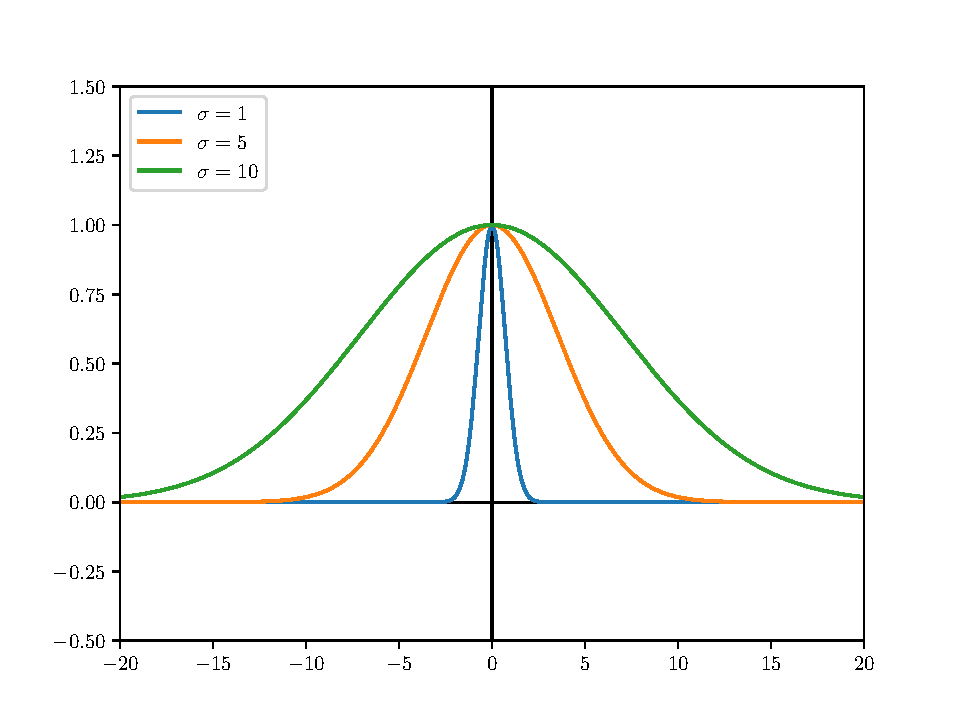
\includegraphics[scale=0.5]{images/exponentail.pdf}
    \caption{Plot of the function $f(x)=exp(-\frac{x^2}{\sigma^2})$ for different values of $\sigma$.}
\end{figure}
First of all, the values are now bound between 0 an 1, regardless of the size of
$\theta$. Second, we can see as the values of the distance get larger, the
function approaches 0 asymtotically. This leads to a really small gradient for
extreme distances. Consequently, the Kernel will initially push the parameters
away from the checkpoint, but when this is achieved, will have little influence
on the loss function. How far the function encourages to distance from the
checkpoint can be controlled by the parameter $\sigma$, which defines the width
of the function and can be tuned as a hyperparamter. As $\sigma$ gets larger,
the function becomes wider. Therefore, the influence of the distance function
will reach further the larger $\sigma$ is.


\subsubsection{Loss function}
This section will show how the distance function from \ref{distance_function} is
combined with the normal loss function. The state of the art loss function for
image classification, which will be used for testing is the cross-entropy-loss
defined as:
\begin{align}
    -\sum_{i} \delta_{yc} log(f(x)_i)
\end{align}
Where $\delta$ is the Kronecker-Delta function defined as:
\begin{align}
    \delta_{xy} =
    \begin{cases}
        1 \textrm{, if } x=y \\
        0 \textrm{ otherwise}
    \end{cases}
\end{align}

To account for the distance term, we just sum it with the cross-entropy-loss:
\begin{align}
    L=\sum_{i} \delta_{yi} log(f(x)_i) + distance(\theta, \theta_c)
\end{align}
Where $\theta_c$ is the checkpoint.
Note that we can do this multiple times, so we can incooperate multiple
checkpoints:
\begin{align}
    L=\sum_{i} \delta_{yi} log(f(x)_i) + \sum_c distance(\theta, \theta_c)
\end{align}
 When computing the derivative for the backpropagation, the sum
decomposes into two terms, so the cross-entropy-loss will be computed the same
as before. Another property we want to control for is the influence of the
distance versus the cross-entropy-loss. When training is in later stages, the
cross-entropy-loss may be very small. If the values of the distance function a
too large in comparison, this would cause the parameters to be updated only
based on the distance, which is undesirable as the performance wouldn't be taken
into account anymore. The same is also true the other way around, if the
distance function is too small, it wouldn't affect training at all. That's why
we introduce a hyperparameters $w$ called weight to control this:
\begin{align}\label{eq:LossDistance}
    L=\sum_{c} \delta_{yc} log(f(x)_c) + w \cdot distance(\theta, \theta_c)
\end{align}

\subsection{Pytorch implementation}

\subsubsection{Checkpoint creation}
To measure the distance, we have to create the checkpoint. The model parameters
in pytorch are stored as matrices for each layer and can be accesed via
$model.parameters()$, which outputs an iterable. We therefore opt to keep this
structure and safe the parameters in a list.
\begin{algorithm}[htbp]
    \caption{Checkpoint}\label{alg:Checkpoint}
    \lstset{language=Python}
    \lstinputlisting{src/createCheckpoint.py}
\end{algorithm}
\newline
First, the checkpoint list is initialized. Then we iterate over the model
parameters. For each layer, we have to clone the parameters in order to create
new variables, and not just pointers to the existing ones. In addition they have
to be detached, to remove connection of the gradient to the model parameters.

\subsubsection{Distance function}
The L2 norm is implemented the follwing way: We iterate over the checkpoint and
the current parameter values. For each layer, we compute the difference, and
then square and add the values to our distance.
\begin{algorithm}[htbp]
    \caption{L2 norm}\label{alg:L2Norm}
    \lstset{language=Python}
    \lstinputlisting{src/L2.py}
\end{algorithm}



\section{Configuration}

\subsection{Library and Training}
The code for the network was written in Python [Version], with the use of
Pytorch as the machine learning library. Data that occured during training was
logged and plotted with Tensorboard. For a detailed overview of the code, see
Appendix [add]. Training was done on the TCML Cluster of the university of Tübingen.

\subsection{Datasets}
Two common datasets were used.
\begin{itemize}
    \item MNIST \\
    MNIST is a classical example of hand-written digits from 0 to 9 that have to
    be classified accordingly. It contains a train set of 60000 and a test set
    of 10000 examples.
    \item CIFAR-10
    This dataset consists of 60000 32x32 colour images with 10 different
    classes. The dataset is seperated into 50000 train and 10000 test images.
    The state of the art accuracy is 97.3\%, reported from Kolesnikov et al.
    (2019). The dataset can be accessed via https://www.cs.toronto.edu/~kriz/cifar.html.
\end{itemize}
\subsection{Networks}
\subsubsection{ResNet}
The Residual Network (ResNet) architecture was first proposed by He et al.
\cite{he2016deep}. The idea of the ResNet was, that it is more easy for a
network to learn the residuals rather than the full representation. Formally,
consider the input $x$. The network transfroms $x$ accoring to $H(x)$. Rather
than letting the network do the full transformation, ResNet produces $H(x)= x
+f(x)$, where $f(x)$ is the residual transformation learned by the network, and
x the identity data which is realized by a skip connection. Beside the assumably
easier to learn representation, ResNet also solves other problems. The issue of
the vanishing gradient as discussed in section [which?] for example is tackled,
as skip connections backpropagate the gradient better to earlier layers of the
network. This allows for deeper networks.

For CIFAR-10, two convolutions are performed and then the residual mapping is
added. After this block is repeated for a number of times, they number of depth
channels is increased. The identity mapping is these layers has to be replaced
by a 1x1 convolution.


\subsubsection{MobileNetV2}
MobileNet was first introduced by Howard et. al \cite{howard2017mobilenets} as a
lightweight neural network for the use on mobile devices. The reduce the
computation effort of the network, the made use of the depth-wise seperable
convolution. Consider a 32x32x3 image of the CIFAR-10 dataset. A traditional 3x3
convolution with a stride and padding of 1 would produce an output of
$\frac{32+2-3}{1}+1$ the shape 32x32x1. To get more channels, we would need more
kernels. For a total of k output channels, we would need to do 3x3x3 x32x32 xk
multiplications. Instead of doing the computation in one kernel, depth-wise
seperable convolution divides it into two kernels. First they perform a
depthwise convolution, where a kernel of 3x3x1 is applied to every channel of
the input, so in this case we end up same size of 32x32x3. To get to k channels,
they use a pointwise convolution across the channels. This is a 1x1x3
convolution, which upscales the image to more channels. So if we want k output
channels, we need k 1x1x3 kernels. The benefit of this technique is that, while
getting the same output size, we only need 32x32 3x3x3 multiplications in the
first step, and 32x32 1x1x3 xk in the second step. This is way less than the
from the beginning.


With the second iteration called MobileNetV2 \cite{sandler2018mobilenetv2}, they
added the concept of inverted residuals or as they call it bottlenecks. The
ideas is, that intermediate representations should be low rather than high
dimensional. The bottleneck layer starts with a matrix with a small number of
depth channels. In the first step, the representation is expanded by a pointwise
convolution, followed by a Relu6. The expansion factor here controls how much
channels the intermediate representation will have. Then a depthwise convolution
is applied as an transformation step, followed again by a Relu6. Finally, a
pointwise convolution is applied again, but this time without a nonlinear
transformation following afterwards. The idea is that when compressing the data
back to a low dimensional space, a nonlinearity would only lead to a loss of
information. Finally, a skip connection from the input to the output is applied
to get a residual mapping from input to output.

Figure x describes the network in detail.

For ImageNet, MobileNetV2 reaches an top-1 accuracy of 72\%, which outperforms
the competitors like MobileNetV1 or ShuffleNet 1.5 while having a similar number
of parameters.


\subsection{Network hyperparameters and training loop}\label{sub:Hyperparameters}
For both networks, the base hyperparameters are the same. Note that these
parameters are only standard configurations and may be changed to investigate
the effects:
\begin{itemize}
    \item Optimization Algorithm \\Stochastic Gradient descent combined with
    Momentum is used. A $\lambda$ of 0.9 is set for Momentum.
    \item Learning rate \\Initially 1e-2
    \item Learning rate scheduler \\ Both step decay and cosine decay are used.
    For step decay, the epochs until a warm restart are divided into 3 parts and
    in every part, the learning rate is decayed by a factor of 0.1. For other
    learning rates, see \ref{res:Learning rate}.
    \item Warm restart \\ A warm restart is performed after 90 epochs (See
    \ref{res:Epochs} for changes). The learning rate is set back up to the
    initial learning rate.
    \item Regularization \\An $L_2$ Regularization as described in chapter
    \ref{sub:Generalization} is used with a factor of 1e-3.
    \item Checkpoints for Distance function \\Every time a warm restart is
    performed, a new checkpoint for the distance function is created.
    \item Number of epochs \\The number of epochs varies. As this is an
    explorative analysis, the training is often run for a large number of
    epochs, to investigate long term changes. Usually an epoch number of 900 is
    used.
\end{itemize}

\begin{comment}
\subsection{Hardware}
\begin{figure}[h]
    \centering
    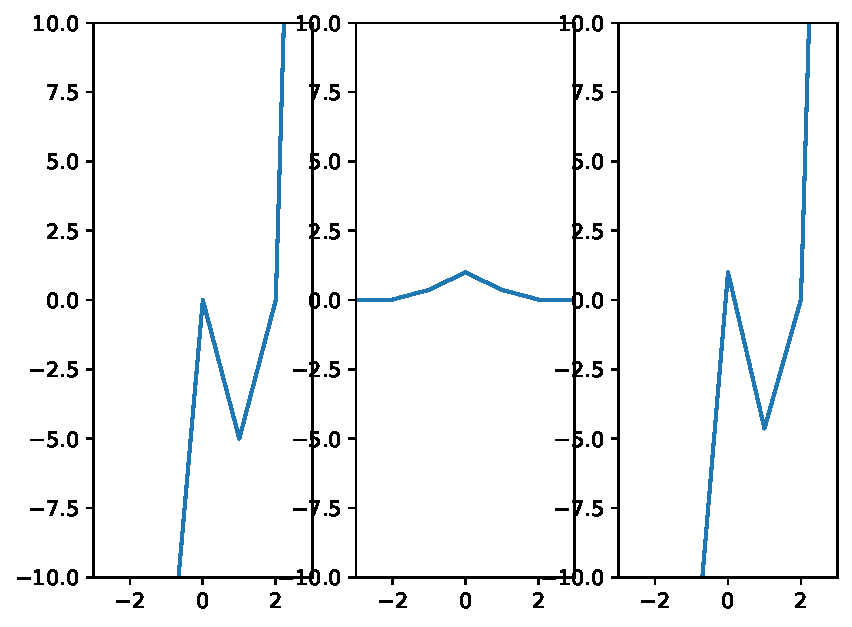
\includegraphics{images/test.pdf}
    \caption{Feature Selection Based on Mutual Information}
    \label{fig:fs_mi}
\end{figure}


\begin{figure}[h]
    \centering
    \includesvg{images/nn.svg}
    \label{fig:fs_mi}
\end{figure}

\end{comment}

